\documentclass[aspectratio=43]{beamer}
\usetheme{Berlin}

\usepackage[czech]{babel}
\usecolortheme{dolphin}
\usepackage{graphicx}
\usepackage{dirtree}
\usepackage{listings}
\usepackage[utf8]{inputenc}
\usepackage{caption}		% popisky

\captionsetup{labelformat=empty}

\defbeamertemplate*{title page}{customized}[1][]
{
  \usebeamerfont{title}\inserttitle\par
  \usebeamerfont{subtitle}\usebeamercolor[fg]{subtitle}\insertsubtitle\par
  \bigskip
  \usebeamerfont{author}\insertauthor\par
  \usebeamerfont{institute}\insertinstitute\par
  \usebeamerfont{date}\insertdate\par
  \usebeamercolor[fg]{titlegraphic}\inserttitlegraphic
}

\hypersetup{unicode}
\hypersetup{breaklinks=true}

\usepackage{color}
\definecolor{pblue}{rgb}{0.13,0.13,1}
\definecolor{pgreen}{rgb}{0,0.5,0}
\definecolor{pred}{rgb}{0.9,0,0}
\definecolor{pgrey}{rgb}{0.46,0.45,0.48}



\title{Židovské město v Třebíči}
\subtitle{Ročníková práce}
\author{Havránek Kryštof 2.E}
\date{\today}
\institute{Gymnázium, Praha 6, Arabská 14}
\setbeamertemplate{sidebar right}{}
\setbeamertemplate{footline}{%
\hfill\textbf{\insertframenumber{}/\inserttotalframenumber}}


\begin{document}
	\begin{frame}[plain]
		\maketitle
	\end{frame}
	\frame{
		\frametitle{Úvod}
		\section{Úvod}
	\begin{itemize}
		\item město na JV Vysočiny
		\item 2 památky UNESCO
		\item obec Podklášteří/Židovské město
		\item proč jsem si práci zvolil?
			\begin{enumerate}
				\item unikátnost těsného soužití Židů a křesťanů
				\item celkový koncept práce -- malé území x dlouhé dějiny
			\end{enumerate}
	\end{itemize}

	}
	\frame{
		\frametitle{Cíl práce}
		\begin{itemize}
			\item shrnout historii města Třebíče
			\item prozkoumat dějiny židovské čtvrti a jejích obyvatel
			\item zmapovat vztahy mezi jednotlivými komunitami
			\item podrobněji popsat důležité budovy židovské čtvrti
		\end{itemize}
	}
	\frame{
		\frametitle{Zdroje}
		\begin{itemize}
			\item knižní
			\item práce poskytnuté židovským muzeem v Třebíči
			\item online
		\end{itemize}
	}

	\frame{
		\frametitle{Město Třebíč}
		\section{Město Třebíč}
		\begin{itemize}
			\item tvoří se okolo kláštera
			\item tržní osady $\Rightarrow$ Podklášteří $\Rightarrow$ 1277?
			\item 12. května 1468 -- Bitva o Třebíč
			\item rekatolizace
			\item národní hnutí
		\end{itemize}
	}
	\frame{
		\frametitle{Židovské město}
		\section{Židovské město}
		\begin{figure}
		\centering
			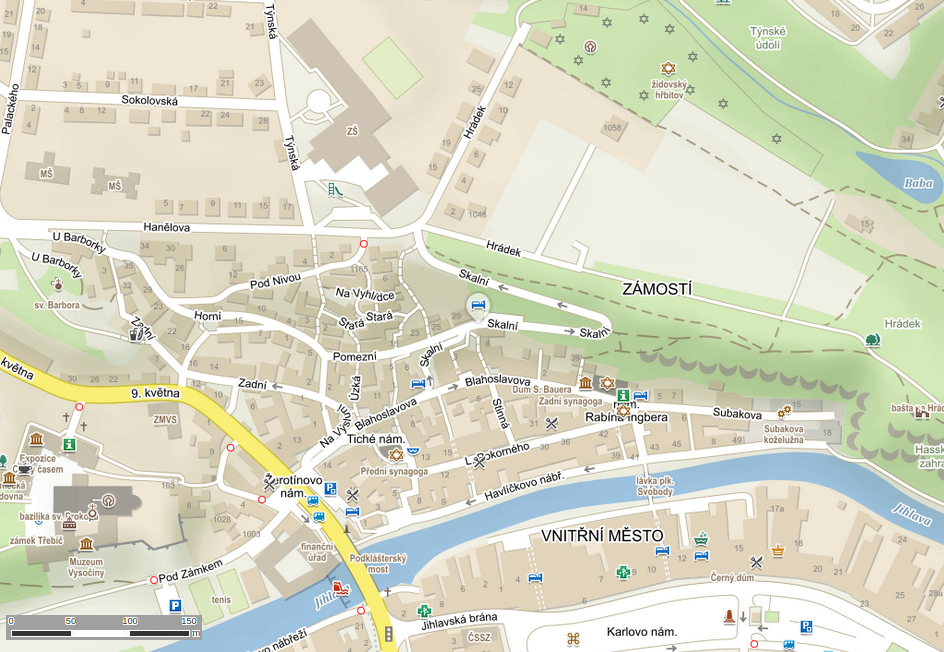
\includegraphics[height=5.8cm]{mapaZidovskehoMesta.png}
    	\caption{Mapa Židovského města\footnotemark}
		\end{figure}
				\footnotetext{\tiny Mapa Židovského města \text{[online]} Mapy.cz. Dostupné z: \url{https://en.mapy.cz/zakladni?x=15.8789945&y=49.2182114&z=17&source=muni&id=5517} \text{[cit. 2020-03-28], zeditováno}}
			}

	\frame{
		\frametitle{Židovské město}
		\begin{itemize}
			\item otázka data založení (933 -- 1410)
			\item Třebíčský machzor -- 1300?
			\item 1338 -- kronikář Neplach
			\item husitské války -- existence není potvrzena
			\item 1547 -- Jan z Perštejna vypověděl Židy, Jetřich Černohorský
			\item 1573 -- 8 rodin
			\item 1629 -- 1. proti--židovské zákony -- Rudolf z Valdštejna
		\end{itemize}
	}
	\frame{
		\frametitle{Židovské město}
		\begin{itemize}
			\item 1. června 1723 -- založeno ghetto Janem Josefem z Valdštejna
			\item Karel VI. -- familiantský zákon, translokační reskript
			\item přírodní i lidmi způsobené pohromy
			\item národní hnutí
			\item 1931 -- Židovská čtvrť sjednocena s Třebíčí
			\item 18. a 19. května 1942 -- deportace
		\end{itemize}
	}
	\frame{
		\frametitle{Židovské město}
		\begin{figure}
		\centering
			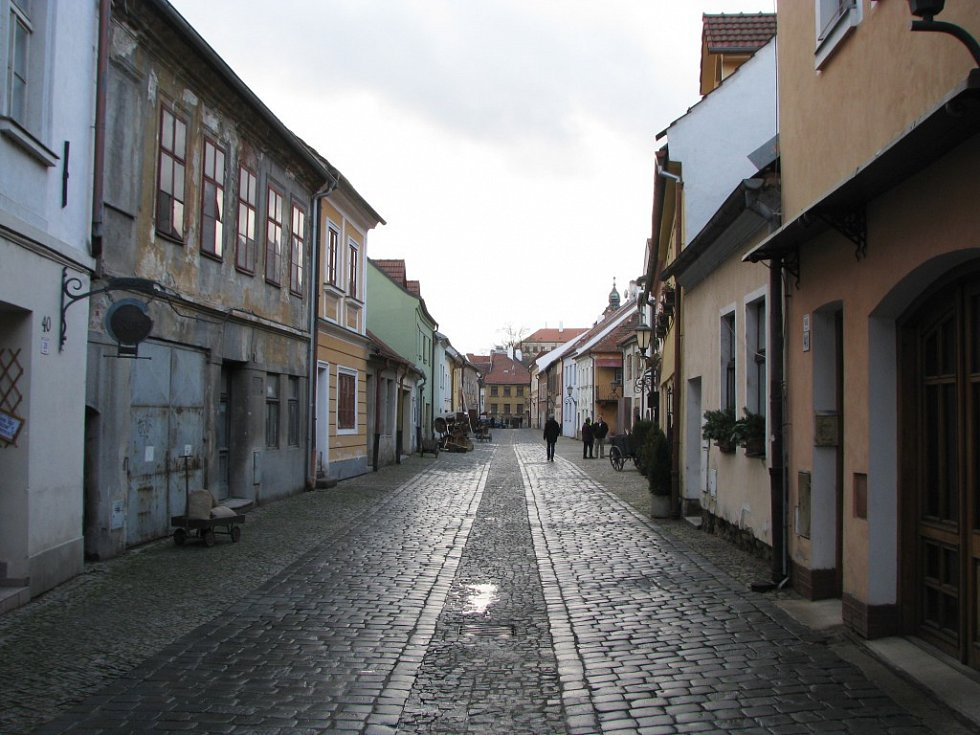
\includegraphics[height=5.8cm]{ulice.jpg}
    	\caption{Ulice Leopolda Pokorného\footnotemark}
		\end{figure}
				\footnotetext{\tiny Ulice Leopolda Pokorného \text{[online]} denik.cz. Dostupné z: \url{https://trebicsky.denik.cz/zpravy\_region/kraj-vysocina-letos-opet-prispeje-mestum-s-pamatkami-unesco-20170315.html} \text{[cit. 2020-06-15]}}
	}
	\frame{
		\frametitle{Židovské město}
		\begin{figure}
		\centering
			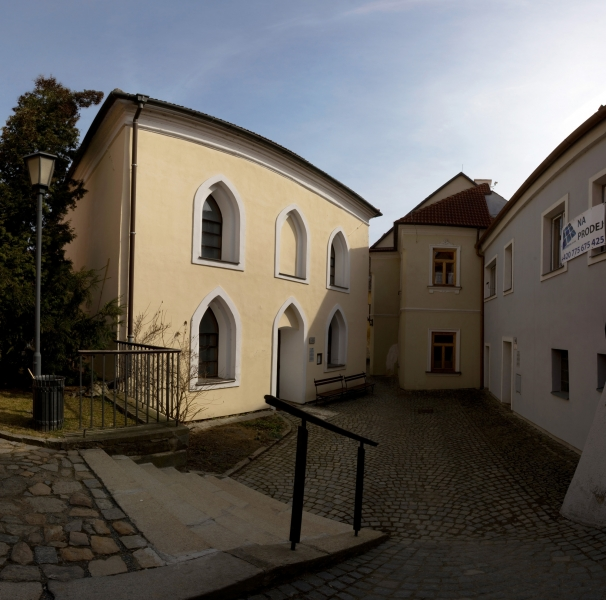
\includegraphics[height=5.8cm]{../img/predniSynagogaBudova}
    	\caption{Přední synagoga \footnotemark}
		\end{figure}
				\footnotetext{\tiny Přední synagoga \text{[online]} MKS Třebíč. Dostupné z: \url{https://www.mkstrebic.cz/data\_5/fotogalerie/15normal.jpg} \text{[cit. 2020-03-26]}}
	}
	\frame{
		\frametitle{Židovské město}
		\begin{figure}
		\centering
			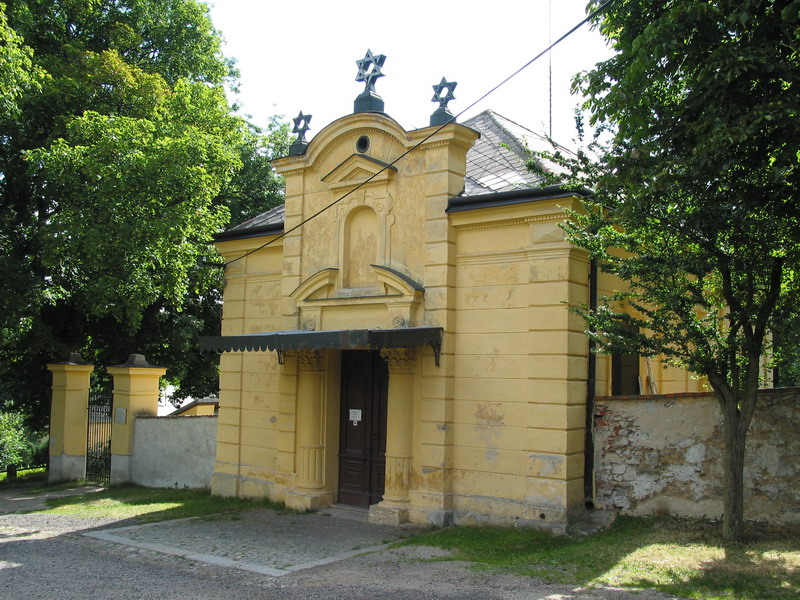
\includegraphics[height=5.8cm]{../img/zidovskyHrbitov.jpg}
    	\caption{Židovský hřbitov\footnotemark}
		\end{figure}
				\footnotetext{\tiny Židovský hřbitov \text{[online]} Město Třebíč. Dostupné z: \url{http://www.mesto-trebic.cz/zidovsky-hrbitov.php} \text{[cit. 2020-03-28]}}
	}
	\frame{
		\frametitle{Závěr}
		\section{Závěr}
		\begin{itemize}
			\item téma není dostatečně probádáno, kvalita zdrojů
			\item nepodařilo se mi město ve dne navštívit
			\item v rámci rozsahu středoškolské práce byl cíl splněn
		\end{itemize}
	}

\end{document}
